%  Typ dokumentu - článek, prezentace aj.
\documentclass[english]{article}

%  Nastaví vstupní a výstupní kódování znaků (encoding) a lokalizace
\usepackage[T1]{fontenc}
\usepackage[utf8]{inputenc}
\usepackage[english,czech]{babel}
\usepackage{icomma}

%  Formát papíru a odsazení od jeho okrajů
\usepackage[letterpaper]{geometry}
\geometry{verbose,tmargin=1.5cm,bmargin=2cm,lmargin=2cm,rmargin=2cm}

%  Umožňuje pracovat s grafikou
\usepackage{graphicx}
\usepackage{bigstrut}
\usepackage{epstopdf}

%  Automaticky odsadí i první paragraf v každé sekci
\usepackage{indentfirst}

%  Umožňuje rozdělovat obsah na více sloupců
\usepackage{multicol}
\usepackage{booktabs}
\usepackage{color}
\definecolor{light-gray}{gray}{0.80}

%  Umožňuje používat hypertextové odkazy, nastavuje jejich barvu a
%  vlastnosti
\usepackage[unicode]{hyperref}
\hypersetup{
colorlinks=true, citecolor=blue, filecolor=blue, linkcolor=blue,
urlcolor=blue
}

%  Umožnění odstranění italiky u jednotek
\newcommand{\unit}[1]{\mathrm{#1}}

%  Formátování stránek, empty = odstraní číslování
% \pagestyle{empty}

%  Řádkování
\linespread{1.2}

%  Lepší zobrazování matematiky (rozšíření sum o \limits atd.)
\everymath{\displaystyle}
\usepackage{amsmath, amsthm, amssymb}

% Umožní psát přes \mathbb{N/R/Q/..} množiny čísel
\usepackage{amssymb}

%  Velikost fontu matematických výrazů v dokumentu lze pro danou
% základního fontu dokumentu upravit pomocí:
% \DeclareMathSizes{X}{Y}{Z}{U} kde:
% X je velikost fontu v dokumentu, pro kterou se matematika upraví
% Y je standartní velikost fontu matematiky
% Z je velikost fontu zmenšených (vnořených výrazů)
% U je velikost fontu ještě více zmenšených (vnořených výrazů).
\DeclareMathSizes{10}{10.5}{9}{9}

%  Nastaví autora, název, datum, skupinu měření apod. (můj vlastní
% příkaz, umožní znovu-použití v dokumentu)
\newcommand{\Author}{David Roesel}
\newcommand{\Coauthor}{Tereza Schönfeldová}
\newcommand{\Institute}{FJFI ČVUT v Praze}
\newcommand{\Subject}{FYZIKÁLNÍ PRAKTIKUM II}
\newcommand{\Group}{7}
\newcommand{\Circle}{ZS 7}
\newcommand{\Title}{Úloha \#9  \\Měření s polarizovaným světlem}
\newcommand{\Date}{10.3.2014}

% Začátek dokumentu - Formátování na výstup
\begin{document}

% Interní proměnné, možno zobrazovat u prezentací, používají se při
% generování pomocí \titlepage apod.
\author{\Author}
\title{\Title}
\date{\Date}

%  Lokalizace některých názvů do češtiny
\renewcommand{\figurename}{Obr.}
\renewcommand{\tablename}{Tab.}
\renewcommand{\refname}{Reference}

% --- Hlavička dokumentu -----------------------------------------------

\setlength{\parindent}{0cm}
\begin{multicols}{2}
\textbf{\Subject \\
        \Institute \\[0.1cm]
%\large  \Title \\[0.5cm]
\Title \\[0.5cm]
}
\begin{tabular}{rlrl}
\large Datum měření: & \Date & \large Skupina: & \Group \\
\large Jméno: & \Author & \large Kroužek:  & \Circle\\
\large Spolupracovala: & \Coauthor &\large Klasifikace:\\
\end{tabular}

\begin{flushright}
\includegraphics[scale=0.28]{../../_meta/fjfi_standart.pdf}
\hspace{0.2cm}
\includegraphics[scale=0.28]{../../_meta/cvut_standart.pdf}
\end{flushright}
\end{multicols}
\hrule
\vspace{0.5cm}

% ----------------------------------------------------------------------


% --- Tělo dokumentu ---------------------------------------------------
\setlength{\parindent}{0.5cm}
\section{Pracovní úkoly}
	  \begin{enumerate}
	\item Při polarizaci bílého světla odrazem na černé skleněné desce proměřte závislost stupně polarizace na sklonu desky a určete optimální hodnotu Brewsterova úhlu. Výsledky zaneste do grafu.
	
	\item Černou otočnou desku nahraďte polarizačním filtrem a proměřte závislost intenzity polarizovaného světla na úhlu otočení analyzátoru (Malusův zákon). Výsledek srovnejte s teoretickou předpovědí a znázorněte graficky.
	
	\item Na optické lavici prozkoumejte vliv čtyř celofánových dvojlomných filtrů, způsobujících interferenci. Vyzkoušejte vliv otáčení polarizátoru, analyzátoru a vliv otáčení dvojlomného filtru mezi zkříženými i rovnoběžnými polarizátory v bílém světle. Zjistěte přímohledným spektroskopem, které vlnové délky se interferencí ruší. Výsledky pozorování popište.
	
	\item Na optické lavici sestavte polostínový polarimetr. Ověřte vliv vzájemného pootočení polarizačních filtrů D a L na citlivost měření úhlu natočení analyzátoru. Při optimálně nastavených filtrech D a L změřte měrnou otáčivost křemíku pro 4 spektrální barvy.
	
	  \end{enumerate}

\section{Vypracování}

	\subsection{Použité přístroje}
		Optická lavice, otočné černé zrcadlo, polarizační filtry s úhlovou stupnicí, multimetr, otočný držák pro dvojlomný vzorek, čtvrtvlnná destička, celofánové dvojlomné filtry, světelný zdroj s matnicí, ruční přímohledný spektroskop, fotočlánek s vodiči, kruhový polarimetr, křemenné destičky tlouštěk 1~mm a 1,5~mm, barevné filtry, irisová clonka, zdroj napětí. 
					
	\subsection{Teoretický úvod}
		
		\subsubsection{Polarizace světla odrazem}
		Dopadá-li světlo na skleněnou desku (nebo jiné rozhraní), část světla se odráží a část se láme do prostředí, které má jiný index lomu. Z části je odražený paprsek lineárně polarizovaný. Stupeň této polarizace bude záviset na úhlu, který odražený paprsek svíral s rovinou zrcadla. Úhel, při kterém je stupeň polarizace nejvyšší, je dán Brewsterovým zákonem (odražený paprsek musí být kolmý na ten dopadající). Při odrazu na rozhraní dvou prostředí (o indexech lomu $n_1$ a $n_2$) platí pro Brewsterův úhel $\theta$ vztah
		\begin{equation}
			\frac{n_2}{n_1} = tg(\theta).
			\label{eq:brewsteruv_uhel}
		\end{equation}
		
		Předpokládáme-li index lomu vzduchu $n_1 = 1$, můžeme pro fit závislosti velikosti vektoru polarizace na úhlu otočení zrcadla použít funkci 
		\begin{equation} \label{eq:brewster_fit}
		P(\vartheta) = \alpha \cdot \frac{ \left( \cos \vartheta - \arcsin \frac{\sin \vartheta}{n} \right)^2 - \left( \cos \vartheta + \arcsin \frac{\sin \vartheta}{n} \right)^2 }{ \left( \cos \vartheta - \arcsin \frac{\sin \vartheta}{n} \right)^2 + \left( \cos \vartheta + \arcsin \frac{\sin \vartheta}{n} \right)^2 } + \delta,
		\end{equation}
		kde parametr $n$ je index lomu skla zrcadla a parametry $\alpha$ a $\delta$ kompenzují nedostatky měření (svícení do soustavy ze stran, příliš mnoho světla v místnosti a nechtěné odrazy).
		
		\begin{figure}[h]
		\centering
		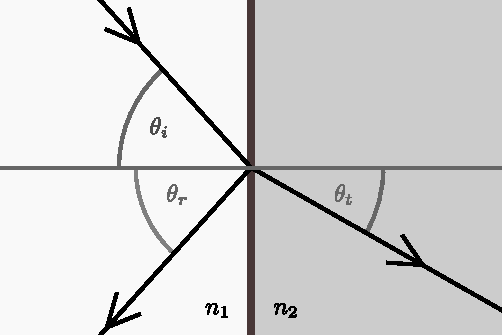
\includegraphics[width=8cm]{att/fresnel.pdf}
		\caption{Odraz a lom světla na rozhraní \cite{bib:slabyji2}}
		\label{fig:fresnel}
		\end{figure}
		
		\subsubsection{Polarizace světla dvojlomem}
		Některé krystalické látky se při průchodu světla chovají jako anizotropní prostředí, tj. jeho optické vlastnosti závisejí na tom, jakým směrem se v krystalu šíří světlo. Existují v nich tedy směry, ve kterých se světlo šíří jako v prostředí s různými indexy lomu. Nepolarizované světlo se tak rozdělí na dva paprsky (řádný a mimořádný). Ten první se řídí Snellovým zákonem a má index lomu $n_o$, zatímco ten druhý se jím neřídí a jeho index lomu $n_e$ závisí na směru šíření světla v krystalu. Tyto dva paprsky jsou lieárně polarizovány v na sebe kolmých rovinách.
		
		\subsubsection{Malusův zákon}
		Pokud necháme procházet lineárně polarizované světlo optickým prvkem schopným polarizovat, uvidíme, že intenzita světla, které projde, závisí na vzájemné úhlové poloze polarizační roviny světelného svazku a polarizátoru, kterým prochází. Polarizátor totiž propustí jen tu složku, která odpovídá jeho polarizační rovině. Intenzita prošlého světla $I'$ se mění podle Malusova zákona
		\begin{equation}
		I(\varphi) = I \cos^2 \varphi + \delta,
		\label{eq:malusuv_zakon}
		\end{equation}
		kde $I$ je intenzita polarizovaného světla dopadajícího na polarizátor, $\varphi$ je úhel svíraný polarizačními rovinami paprsku a polarizátoru a $\delta$ je posun kompenzující nedostatky měření.
		
		\subsubsection{Interference rovnoběžně polarizovaného světla}
		V případě, že lineárně polarizované světlo prochází dvojlomnou destičkou, rozdělí se na dva paprsky, jejichž rychlost šíření je rozdílná, a tak i z destičky vychází s jistý dráhovým rozdílem. Dráhový rozdíl obou paprsků závisí na tloušťce destičky a rozdílu význačných indexů lomu a tím pádem na vlnové délce světla. Pokud procházejí oba paprsky polarizátorem, projdou jen složky odpovídající jeho polarizační rovině, čímž dojde k interferenci - některé barvy se vyjasňují a jiné zeslabují.
		
		\subsubsection{Rotační polarizace}
		U některých látek (například u křemenné destičky vyříznuté kolmo k optické ose) pozorujeme schopnost stáčet rovinu polarizace. Takovéto látky rozlišujeme na pravo- a levotočivé. To, jak moc se rovina polarizace stáčí, závisí na vlnové délce polarizovaného světla (kratším vlnovým délkám odpovídá větší otočení) a přímo úměrně na tloušťce destičky. Látky klasifikujeme takzvanou měrnou otáčivostí, tedy otočení polarizační roviny způsobené vrstvou látky o jednotkové tloušťce.
		
		\subsubsection{Stupeň polarizace}
		Skutečné světlo není nikdy úplně koherentní a rozlišovací doba přístroje není shodná s koherenčními dobami. Proto pro určení stupně polarizace používáme takzvané Stokesovy parametry:
		
		\begin{equation} \label{eq:stokesovy_parametry}
		P_1 = \frac{\langle E^2_x \rangle_r - \langle E_y^2 \rangle_r}{\langle E^2_x \rangle_r + \langle E_y^2 \rangle_r}, \qquad P_2 = \frac{\langle 2 E_x E_y \rangle_r}{\langle E^2_x \rangle_r + \langle E_y^2 \rangle_r}, \qquad P_3 = \frac{\langle 2E_x (\omega t - \pi/2) E_y (\omega t) \rangle_r}{\langle E^2_x \rangle_r + \langle E_y^2 \rangle_r},
		\end{equation}
		které charakterizují tzv. částečně polarizované světlo.
		
		Velikost vektoru $\vec{P} = (P_1, P_2, P_3)$ představuje stupeň polarizace světla a může nabývat hodnot od nuly do jedné včetně: nepolarizovanému světlu odpovídá $|\vec{P}| = 0$, úplně polarizovanému naopak $|\vec{P}| = 1$.
		
		Při zjišťování polarizace, tedy Stokesových parametrů, změříme 4 různé intenzity:
		\begin{enumerate}
		 \item Při polarizátoru nastaveném na 0 $^\circ$ chceme zjistit $\left\langle {E_x^2 } \right\rangle _{r}$.
		 \item Při polarizátoru nastaveném na 90 $^\circ$ chceme zjistit $\left\langle {E_y^2 } \right\rangle _{r}$.
		 \item Při polarizátoru nastaveném na 45 $^\circ$ chceme zjistit $\frac{1}{2}\left\langle {E_x^2 } \right\rangle _{r} + \frac{1}{2}\left\langle {E_y^2 } \right\rangle _{\tau} + \left\langle {E_x E_y } \right\rangle _{r}$.
		 \item Při polarizátoru nastaveném na 45 $^\circ$ a čtvrtvlnovou destičkou chceme zjistit \newline $\frac{1}{2}\left\langle {E_x^2 } \right\rangle _{r} + \frac{1}{2}\left\langle {E_y^2 } \right\rangle _{r} + \left\langle {E_{x}(\omega t - \pi/2 ) E_{y}(\omega t)} \right\rangle _{r}$.
		\end{enumerate}
		
		Z těchto hodnot již zvládneme dopočítat Stokesovy parametry pomocí vzorce  (\ref{eq:stokesovy_parametry}).




	\subsection{Postup měření}
		\subsubsection{Určení Brewsterova úhlu}
			Schéma nastavení aparatury je na Obr. \ref{fig:brewsteruv_uhel}. Vzhledem k tomu, že měření závisí na natočení zrcadla vůči optické lavici, museli jsme nejprve provést kalibraci podle návodu \cite{bib:zadani}. Před černé zrcadlo jsme na lavici umístili kalibrační tyčku s výřezem a na druhý konec lavice jsme dali tyčku s hrotem. Následně jsme se snažili nastavit zrcadlo tak, aby byl odraz hrotu v zákrytu, tedy aby rovina zrcadla byla přesně kolmá na osu optické lavice. Následně jsme zaaretovali pozici zrcadla a po zbytek experimentu používali pouze otočný kloub se stupnicí.

			\begin{figure}[h!]
			\centering
			\includegraphics[width=9cm]{att/brewsteruv_uhel.pdf}
			\caption{Sestava pro pokus na určení Brewsterova úhlu; A~--~Optická lavice, B~--~Světelný zdroj, C~--~Otočné černé zrcadlo, D~--~Polarizační filtr, E~--~Čtvrtvlnová destička, F~--Fotočlánek, G~--~Multimetr, K~--~Matnice, P~--~Irisová clonka. Převzato z \cite{bib:zadani}.}
			\label{fig:brewsteruv_uhel}
			\end{figure}

			Jednotlivé prvky na optické lavici jsme sestavili podle schématu na Obr. \ref{fig:brewsteruv_uhel}. Mezi jednotlivými prvky jsme volili minimální vzdálenost a snažili se je co nejpřesněji srovnat do jedné výšky. Vlastní měření probíhalo odečítáním hodnot napětí na fotočlánku, které zobrazoval k němu připojený multimetr. Napětí (tedy nepřímo intenzitu dopadajícího světla) jsme sledovali v závislosti na úhlu natočení zrcadla a pro každý úhel jsme udělali čtyři měření s následujícím nastavením:
			\begin{enumerate}
			\item s analyzátorem nastaveným na 0 $^\circ$
			\item s analyzátorem nastaveným na 90 $^\circ$
			\item s analyzátorem nastaveným na 45 $^\circ$
			\item s analyzátorem nastaveným na 45$^\circ$ \ a čtvrtvlnovou destičkou mezi analyzátorem a irisovou clonou,
			\end{enumerate}
			přičemž roli polarizátoru plnilo černé zrcadlo a jako analyzátor fungoval polarizační filtr. Z hodnot naměřených tímto způsobem můžeme určit Stokesovy parametry (\ref{eq:stokesovy_parametry}).

			Hodnoty napětí jsme zaznamenávali od 40 $^\circ$ do 72,5 $^\circ$ s krokem 5 $^\circ$ na okrajích, 2,5 $^\circ$ v průběhu a v okolí předpokládaného maxima 58 $^\circ$ (\ref{eq:brewsteruv_uhel}) jsme se snažili i o krok 1,25 $^\circ$. Pokaždé, když jsme natočili zrcadlo, bylo třeba nastavit zdroj tak, aby byla splněna podmínka zákonu odrazu. Vždy, když jsme nastavili zrcadlo na úhel $\alpha$, museli jsme nastavit zdroj na úhel $270-\alpha$ $^\circ$.


		\subsubsection{Ověření Malusova zákona}
			Schéma nastavení aparatury je na Obr. \ref{fig:malusuv_zakon}. Stejně jako v minulém úkolu jsme jednotlivé prvky na optické lavici umístili co nejblíže k sobě a vyrovnali co nejlépe jejich výšku či orientaci. Polarizátor blíže ke zdroji světla jsme nejprve nastavili co nejpřesněji na nulu a během měření jsme měnili úhel pouze na přesnějším polarizačním filtru dále od zdroje. Analogicky minulému úkolu jsme zaznamenávali napětí na fotočlánku, tentokrát však v závislosti na rozdílu úhlů obou polarizátorů. Za konstantní polohy polarizátoru jsme tak měnili na analyzátoru úhel od -95 do +95 $^\circ$ s krokem 5 $^\circ$.
			
			\begin{figure}[h!]
			\centering
			\includegraphics[width=9cm]{att/malusuv_zakon.pdf}
			\caption{Sestava pro ověření Malusova zákona; A~--~Optická lavice, B~--~Světelný zdroj, D~--~Polarizační filtr, F~--Fotočlánek, G~--~Multimetr, K~--~Matnice. Převzato z \cite{bib:zadani}.}
			\label{fig:malusuv_zakon}
			\end{figure}

		\subsubsection{Interference v lineárně polarizovaném světle}
			Schéma nastavení aparatury je na Obr. \ref{fig:interference}. Vše jsme nastavili podle něj, až na to, že jsme vynechali přímohledný spektroskop (J) a kondenzor (I), z důvodu posunutého krystalu ve spektroskopu. Jevy jsme pozorovali nakonec i bez dalekohledu, jelikož byly vidět dostatečně dobře. 
			
			\begin{figure}[h!]
			\centering
			\includegraphics[width=9cm]{att/interference.pdf}
			\caption{Sestava pro zkoumání interference v lineárně polarizovaném světle; A~--~Optická lavice, B~--~Světelný zdroj, D~--~Polarizační filtr, H~--~Otočný držák na dvojlomný vzorek, I~--~Kondenzor, J~--~Přímohledný spektroskop. Převzato z \cite{bib:zadani}.}
			\label{fig:interference}
			\end{figure}
			
		\subsubsection{Optická aktivita křemíku}
			Schéma nastavení aparatury je na Obr. \ref{fig:opticka_aktivita}. Nastavování aparatury vyžadovalo vyzkoušet několik vzdáleností jednotlivých optických prvků. Cílem tohoto měření bylo určit měrnou otáčivost křemene pro čtyři různé vlnové délky. Pro každou z nich jsme postupovali podle následujícího postupu:
			\begin{enumerate}
				\item Do přihrádky u matnice jsme zasunuli barevný filtr odpovídající vlnové délky.
				\item Bez křemenné destičky jsme nejdříve nastavili polarizátor D na -90 $^\circ$ a poloviční polarizační filtr L na +85 $^\circ$.
				\item V zorném poli dalekohledu v tuto chvíli bylo možné pozorovat dvě poloviny, jejichž poměr jasů se se změnou natočení polarizátoru O měnil.
				\item Následně jsme nastavili polarizátor O tak, aby byl jas obou polovin stejný a jeho nastavení jsme si zaznamenali.
				\item Poté jsme na odpovídající místo vložili zkoumaný vzorek a znovu našli polohu polarizátoru O tak, aby byl jas obou polovin vyrovnaný, a tuto hodnotu jsme zaznamenali. 
				\item Pro každý ze čtyř barevných filtrů jsme předchozí body opakovali s destičkami o tloušťkách 1 a 1,5~mm.
			\end{enumerate}
			
			\begin{figure}[h!]
			\centering
			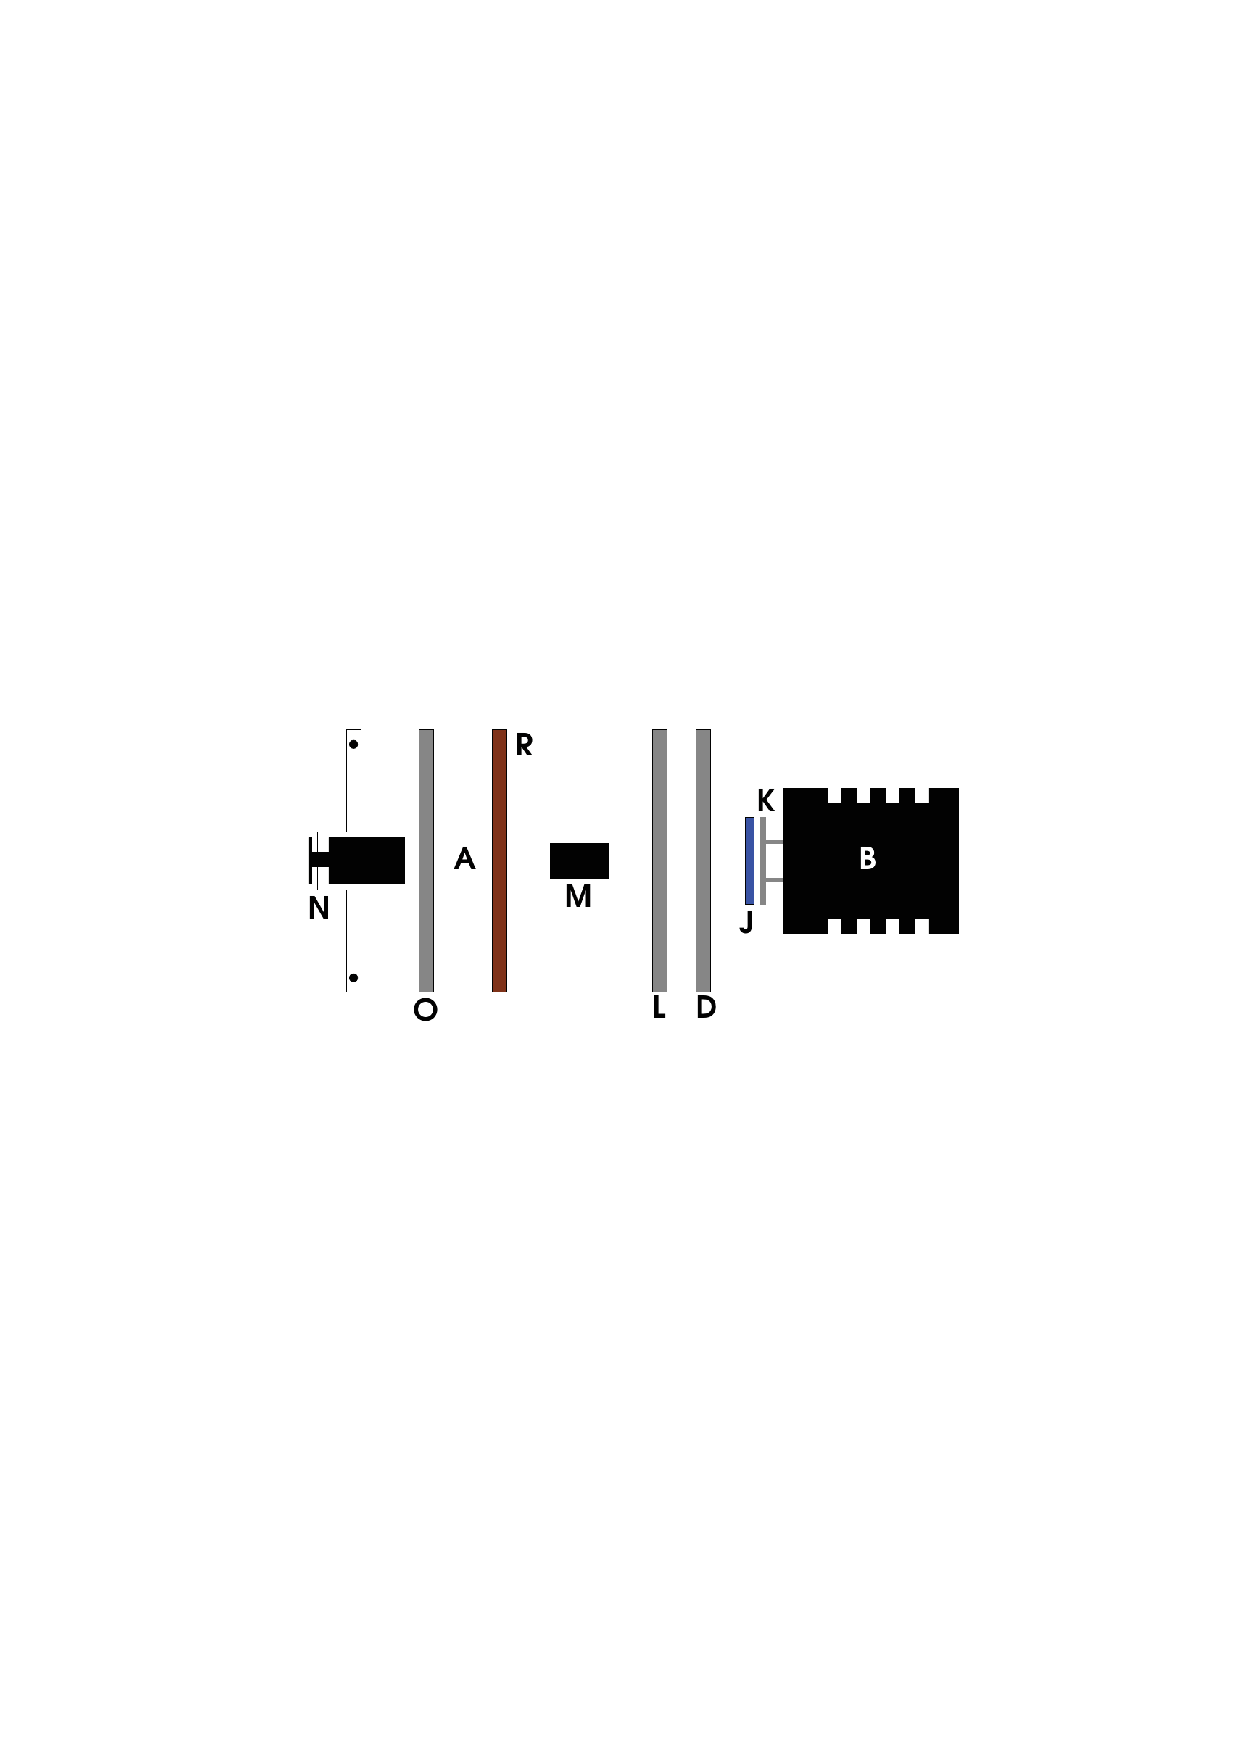
\includegraphics[width=10cm]{att/opticka_aktivita.pdf}
			\caption{Sestava pro měření optické aktivity křemíku; A~--~Optická lavice, B~--~Světelný zdroj, D~--~Polarizační filtr, J~--~Barevný filtr, L~--~Poloviční polarizační filtr, M~--~Spojná čočka, N~--~Dalekohled zaostřený na nekonečno, O~--~Polarizační filtr s jemně dělenou stupnicí a noniem, R~--~Zkoumaný vzorek. Převzato z \cite{bib:zadani}.}
			\label{fig:opticka_aktivita}
			\end{figure}

	\subsection{Naměřené hodnoty}
		Naměřené hodnoty z určování Brewsterova úhlu jsou vyneseny v grafu na Obr. \ref{fig:g_brewsteruv_uhel} a také v Tab. \ref{tab:brewsteruv_uhel}. Nejvyšší hodnotu jsme u této úlohy naměřili při 
		\begin{equation}
			\theta_{max} = (57,5 \pm 2,5)~^\circ,
		\end{equation}
		přičemž závislost, kterou jsme fitovali, nabývá svého maxima v bodě
		\begin{equation}
			\theta_{fit} = (55,8 \pm 2,5)~^\circ.
		\end{equation}
		Námi provedený fit odpovídá hodnotě indexu lomu skleněného zrcadla 
		\begin{equation}
			n_2 = (1,451 \pm 0,008).
		\end{equation}
		
		Hodnoty naměřené při ověřování Malusova zákona jsou vyneseny v grafu na Obr. \ref{fig:g_malusuv_zakon} a také v Tab. \ref{tab:malus}. 

		Výsledky měření interference v lineárně polarizovaném světle jsou v Tab. \ref{tab:barvicky}. 
		
		Hodnoty naměřené při zkoumání optické aktivity křemíku jsou v Tab. \ref{tab:kremik}.

	\subsection{Diskuse}
			\subsubsection{Určení Brewsterova úhlu}
				Podle vzorce (\ref{eq:brewsteruv_uhel}) a u úlohy zjištěné hodnoty indexu lomu skleněného zrcadla $n_{z}=1,6$ jsme před vlastním měření spočítali odhad pro Brewsterův úhel jako $\theta_B=58~^\circ$. My jsme během měření dosáhli nejvyšší hodnoty napětí při úhlu $\theta=57,5~^\circ$, což je vzhledem k přesnosti $2,5~^\circ$ hodnota odpovídající teoretickému odhadu. Méně přesně pak vyšel fit, který jsme zkoušeli použít. Z proložení jsme získali hodnotu okolo $56~^\circ$, což při uvažování chyby určení úhlu není příliš daleko od našeho předpokladu. Měření by se dalo velmi zpřesnit použitím jemnějšího úhlového měřítka (obzvláště pak toho, podle kterého se nastavoval zdroj světla). V okolí maxima jsme se snažili měřit v menších intervalech, než nám dovolovaly naše rozlišovací schopnosti, a to se projevilo na hodnotě maxima fitu. Při výpočtech nám navíc vycházely pro některé složky (velmi mírně, ale přece) záporné hodnoty a bylo by záhodno tento jev nějak kompenzovat. Další část pokusu, která by se dala zlepšit, byl fakt, že všech úhlech, obzvláště pak v těch krajních, svítil zdroj zcela evidentně nejen na zrcadlo, takže docházelo k nechtěným odrazům.
				
			\subsubsection{Ověření Malusova zákona}
				Malusův zákon se nám podařilo ověřit úspěšně. Pro úspěšné znázornění závislosti bylo potřeba k vykreslované funkci přičíst parametr $\delta$, který jsme určili jako hodnotu signálu v momentu, kdy na sebe oba dva polarizační filtry byly kolmé. V tu dobu by soustavou nemělo procházet žádné světlo a signál, který fotočlánek přijímal, byl tedy působen světelným pozadím v místnosti nebo nechtěnými odrazy. Jako počáteční intenzitu pro teoretickou závislost bereme nejvyšší naměřenou hodnotu, což může vést k podsazení celé závislosti podle toho, jak pod- či nadhodnocená tato jedna hodnota byla. Měření by šlo zpřesnit důkladnějším zatemněním místnosti, dokonalejší aparaturou nebo lepším použitím irisové clonky. Měření svou přesností i výsledky odpovídá závěrům z předchozí úlohy praktika, ve které jsme se věnovali studiu mikrovln.
				
			\subsubsection{Interference v lineárně polarizovaném světle}
				Tento jev jsme prozkoumali úspěšně. Nutno říci, že jsou veškeré výsledky spíše orientačního charakteru a nelze z nich činit žádné závěry. Zajímavé bylo, že v některých případech nebyla v průhledu vidět pouze jedna barva, ale některé kusy byly zbarveny barvou druhou. To, že byl rozbitý přímohledný spektroskop, ještě více ztížilo možnost úlohu nějak více analyzovat. Interferenci jsme ovšem pozorovali a úlohu se nám podařilo provést úspěšně. 
				
			\subsubsection{Optická aktivita křemíku}
				Tento pokus již sice obsahoval hodnoty, které se daly měřit, byl však velmi subjektivní a naměřené hodnoty nebudou ani z daleka přesné. Měření spočívá ve stanovení momentu, kdy jsou obě poloviny průhledu stejně jasné. V závislosti na pozorovateli a zvoleném filtru se ale tyto hodnoty lišily v řádu desítek stupňů. I přesto ale hodnoty z měření pro obě tloušťky byly překvapivě blízko sobě. Statistické chyby u nich nejsou jistě odpovídající, jelikož vznikly jako chyby aritmetického průměru dvou hodnot a reálná chyba měření se bude pohybovat v řádu desítek procent naměřené hodnoty.  
				
			
\section{Závěr}
Při polarizaci bílého světla odrazem na černé skleněné desce jsme proměřili závislost stupně polarizace na sklonu desky a určili optimální hodnotu Brewsterova úhlu. Výsledky jsme zanesli do grafu a proložili předpokládanou závislostí s korekcí pro nedokonalé podmínky. 

Černou otočnou desku jsme nahradili polarizačním filtrem a proměřili závislost intenzity polarizovaného světla na úhlu otočení analyzátoru, čímž jsme ověřili Malusův zákon. Výsledek jsme srovnali s teoretickou předpovědí a graficky znázornili.

Na optické lavici jsme prozkoumali vliv čtyř celofánových dvojlomných filtrů, způsobujících interferenci. Vyzkoušeli jsme vliv otáčení polarizátorem, analyzátorem a dvojlomným filtrem v bílém světle. Z důvodu jeho nefunkčnosti jsme přímohledným spektroskopem nezjistili, které vlnové délky se interferencí ruší, ale zapsali jsme výsledky svých pozorování.

Nakonec jsme na optické lavici sestavili polostínový polarimetr a ověřili vliv vzájemného pootočení dvou polarizačních filtrů na citlivost měření úhlu natočení analyzátoru. Při těchto filtrech v optimálním nastavení jsme změřili měrnou otáčivost křemíku pro 4 spektrální barvy a výsledky zapsali.


\section {Použitá literatura}
% --- Literatura a reference -------------------------------------------
\begingroup
\renewcommand{\section}[2]{}

\begin{thebibliography}{9}
\bibitem{bib:zadani} Kolektiv KF, \emph{Návod k úloze: Měření s polarizovaným světlem} [Online], [cit. \today] \newline http://praktikum.fjfi.cvut.cz/pluginfile.php/422/mod\_resource/content/2/Polarizace\_2012.pdf

\bibitem{bib:slabyji2} Josh Lee, \emph{Fresnel.svg} [Online], [cit. \today] \newline
http://commons.wikimedia.org/wiki/File:Fresnel.svg

%\bibitem{bib:h3} Petr Chaloupka, \emph{Jak zpracovávat data} [Online], [cit. \today] \newline  https://dl.dropboxusercontent.com/u/11296940/zfm/h3.pdf

%\bibitem{bib:navody} Kolektiv KF, \emph{Návody k přístrojům} [Online], [cit. \today] \newline http://praktikum.fjfi.cvut.cz/documents/chybynav/navody-o.pdf

\bibitem{bib:chyby} Kolektiv KF, \emph{Chyby měření} [Online], [cit. \today] \newline http://praktikum.fjfi.cvut.cz/documents/chybynav/chyby-o.pdf

%\bibitem{bib:ctverce} Kolektiv KACH UPOL, \emph{Hodnocení analytických výsledků} [Online], [cit. \today] \newline http://ach.upol.cz/ucebnice/hodnoceni7.htm

%\bibitem{bib:tabulky} J. Mikulčák a kol., Matematické, fyzikální a chemické tabulky \& vzorce. Prometheus,
%Praha 2009.\newline
%ISBN 978-80-7196-264-9

%\bibitem{bib:repo} Kolektiv autorů, \emph{Repozitář zdrojů k praktiku} [Online], [cit. \today] \newline  http://github.com/roesel/praktika

\end{thebibliography}
\endgroup
% ----------------------------------------------------------------------
\setcounter{equation}{0}
\numberwithin{equation}{section}
%\clearpage
\part{Přílohy}

\section{Domácí příprava}
	Domácí příprava je přiložena k protokolu.
%\clearpage
\section{Statistické zpracování dat}
	Pro statistické zpracování využíváme aritmetického průměru:
	\begin{equation} \label{eq:aritmeticky_prumer}
	\overline{x} = \frac{1}{n}\sum\limits_{i=1}^{n}x_i,
	\end{equation}
	
	jehož chybu spočítáme jako 
	\begin{equation} \label{eq:chyba_aritmetickeho_prumeru}
	\sigma_0 = \sqrt{\frac{1}{n(n-1)} \sum\limits_{i=1}^{n}\left( x_i - \overline{x} \right)^2 },
	\end{equation}
	
	kde $ x_i $ jsou jednotlivé naměřené hodnoty, $ n $ je počet měření, $ \overline{x} $ aritmetický průměr a $ \sigma_0 $ jeho chyba \cite{bib:chyby}.
%	
%Při nepřímém měření počítáme hodnotu s chybou dle následujících vztahů:
%	\begin{equation}
%	u = f(x, y, z, \ldots),
%	\end{equation}
%	\begin{displaymath}
%	x = (\overline{x} \pm \sigma_x), \qquad
%	y = (\overline{y} \pm \sigma_y), \qquad
%	z = (\overline{z} \pm \sigma_z), \qquad
%	\ldots,
%	\end{displaymath}
%	
%	kde $ u $ je veličina, kterou určujeme nepřímo z měřených veličin $ x, y, z, \ldots $ 
%	
%	Pak
%	\begin{displaymath}
%	\overline{u} = f(\overline{x}, \overline{y}, \overline{z}, \ldots),
%	\end{displaymath}
%	\begin{equation}\label{eq:chyba_neprime_mereni}
%	\sigma_u = \sqrt{\left( \frac{\partial f}{\partial x} \right)^2 \sigma^2_x + \left( \frac{\partial f}{\partial y} \right)^2 \sigma^2_y + \left( \frac{\partial f}{\partial z} \right)^2 \sigma^2_z + \ldots},
%	\end{equation}
%	\begin{displaymath}
%	u = (\overline{u} \pm \sigma_ u).
%	\end{displaymath}
%%	
%V případě, že máme několik různě přesných měření stejné veličiny, používáme vztah pro vážený průměr:
%	\begin{equation} 
%	\bar{x}=\frac{\sum\limits_{i=1}^{n}p_{i}x_{i}}{\sum\limits_{i=1}^{n}p_{i}},
%	\end{equation}
%	
%	kde $\bar{x}$ je vážený průměr, $x_{i}$ jsou jednotlivá měření a pro $p_{i}$ platí
%	 
%	\begin{equation}
%	p_{i}=\frac{1}{\sigma_{i}^{2}},
%	\end{equation}
%	
%	kde $\sigma_{i}$ jsou jednotlivé chyby daných měření.
%	 
%	Celkovou chybu tedy vypočítáme ze vztahu
%	\begin{equation} \label{eq:vazeny_prumer}
%	\sigma_{0}=\sqrt{\frac{1}{\sum\limits_{i=1}^{n}p_{i}}}.
%	\end{equation}
%
%\subsubsection{Metoda nejmenších čtverců}
%Snažíme-li se metodou nejmenších čtverců proložit data lineární závislostí $Y_i = ax_i+b$, dosazujeme hodnoty $x_i, y_i$ a snažíme se najít parametry $a$ a $b$ tak, aby byl součet všech kvadratických odchylek $\Delta Y_i^2$ minimální. Toho dosáhneme pomocí následujících vzorců \cite{bib:ctverce} :
%\begin{equation}\label{eq:ctverce_a}
%		a = \frac{n\sum\limits_{i=1}^{n}{x_i y_i}  - \sum\limits_{i=1}^{n}{x_i}\sum\limits_{i=1}^{n}{y_i}}{n\sum\limits_{i=1}^{n}{x_i^2}  - \left(\sum\limits_{i=1}^{n}{x_i}\right)^2}, \qquad \qquad
%		\sigma_a = \sqrt{\frac{n\sum\limits_{i=1}^{n}{(y_i - Y_i)^2} }{(n-2)\left(\sum\limits_{i=1}^{n}{x_i^2}  - \left(\sum\limits_{i=1}^{n}{x_i}\right)^2\right)}},
%\end{equation}
%
%\begin{equation}\label{eq:ctverce_b}
%		b = \frac{\sum\limits_{i=1}^{n}{x_i^2} \sum\limits_{i=1}^{n}{y_i}  - \sum\limits_{i=1}^{n}{x_i}\sum\limits_{i=1}^{n}{x_i y_i}}{n\sum\limits_{i=1}^{n}{x_i^2}  - \left(\sum\limits_{i=1}^{n}{x_i}\right)^2}, \qquad \qquad
%		\sigma_b = \sqrt{\frac{\sum\limits_{i=1}^{n}{x_i^2}\sum\limits_{i=1}^{n}{(y_i - Y_i)^2} }{n(n-2)\left(\sum\limits_{i=1}^{n}{x_i^2}  - \left(\sum\limits_{i=1}^{n}{x_i}\right)^2\right)}}.
%\end{equation}
	
\clearpage
\subsection{Tabulky a grafy}

		\begin{figure}[h!]
		\begin{center}
		    \vspace*{-1cm}
			\includegraphics[width=\linewidth]{../gnuplot/1_pola.pdf}
		    \vspace*{-2cm}
			\caption{Graf závislosti velikosti vektoru polarizace $|\vec{P}|$ na úhlu natočení černého zrcadla $\theta$. Naměřená data jsou proložena závislostí podle (\ref{eq:brewster_fit}).}
			\label{fig:g_brewsteruv_uhel}
		\end{center}
		\end{figure}
		
		% Table generated by Excel2LaTeX from sheet 'Brewsteruv uhel'
		\begin{table}[htbp]
		  \centering
		    \begin{tabular}{|r|r|r|r|r|r|r|r|r|}
		    \hline
		    \boldmath{}\textbf{$\theta$ [$\unit{^\circ}$]}\unboldmath{} & \boldmath{}\textbf{$|\vec{P}|$ [-]}\unboldmath{} & \boldmath{}\textbf{$P_1$ [-]}\unboldmath{} & \boldmath{}\textbf{$P_2$ [-]}\unboldmath{} & \boldmath{}\textbf{$P_3$ [-]}\unboldmath{} & \boldmath{}\textbf{$U_1$ [mV]}\unboldmath{} & \boldmath{}\textbf{$U_2$ [mV]}\unboldmath{} & \boldmath{}\textbf{$U_3$ [mV]}\unboldmath{} & \boldmath{}\textbf{$U_4$ [mV]}\unboldmath{} \bigstrut\\
		    \hline
		    40,00 & 0,218 & 0,20  & -0,02 & -0,09 & 27,4  & 18,3  & 22,3  & 20,9 \bigstrut\\
		    \hline
		    45,00 & 0,275 & 0,26  & -0,01 & -0,10 & 33,0  & 19,5  & 25,9  & 23,7 \bigstrut\\
		    \hline
		    50,00 & 0,312 & 0,30  & -0,01 & -0,09 & 37,5  & 20,3  & 28,6  & 26,2 \bigstrut\\
		    \hline
		    52,50 & 0,320 & 0,31  & -0,01 & -0,08 & 44,0  & 23,2  & 33,4  & 30,9 \bigstrut\\
		    \hline
		    55,00 & 0,325 & 0,32  & 0,00  & -0,08 & 47,3  & 24,6  & 36,1  & 33,2 \bigstrut\\
		    \hline
		    56,25 & 0,324 & 0,32  & 0,01  & -0,05 & 41,3  & 21,3  & 31,5  & 29,6 \bigstrut\\
		    \hline
		    57,50 & 0,329 & 0,32  & 0,01  & -0,09 & 48,6  & 25,2  & 37,4  & 33,7 \bigstrut\\
		    \hline
		    57,75 & 0,319 & 0,32  & 0,02  & -0,05 & 48,0  & 25,0  & 37,2  & 34,7 \bigstrut\\
		    \hline
		    60,00 & 0,313 & 0,31  & 0,03  & -0,06 & 57,1  & 30,3  & 44,8  & 41,2 \bigstrut\\
		    \hline
		    62,50 & 0,297 & 0,29  & 0,02  & -0,06 & 68,4  & 37,7  & 53,9  & 49,7 \bigstrut\\
		    \hline
		    65,00 & 0,285 & 0,27  & 0,01  & -0,09 & 73,0  & 41,9  & 58,3  & 52,4 \bigstrut\\
		    \hline
		    67,50 & 0,257 & 0,24  & 0,01  & -0,08 & 74,9  & 45,5  & 61,1  & 55,4 \bigstrut\\
		    \hline
		    70,00 & 0,220 & 0,21  & 0,01  & -0,07 & 84,1  & 55,0  & 70,5  & 64,9 \bigstrut\\
		    \hline
		    72,50 & 0,197 & 0,18  & 0,03  & -0,07 & 89,8  & 62,1  & 78,0  & 70,7 \bigstrut\\
		    \hline
		    \end{tabular}%
		     \caption{Naměřené hodnoty pro určování Brewsterova úhlu; $\theta$ je úhel dopadu, $|\vec{P}|$ stupeň polarizace, $P_{1-3}$ Stokesovy parametry a $U_{1-4}$ napětí při každé ze 4 konfigurací popsaných v postupu. Hodnoty napětí jsme brali vzhledem k chybě $\sigma_\theta = 2,5~^\circ$ jako absolutně přesné.  }
		  \label{tab:brewsteruv_uhel}
		\end{table}%				
		
		\begin{figure}[h!]
		\begin{center}
		    \vspace*{-1cm}
			\includegraphics[width=\linewidth]{../gnuplot/2_malus.pdf}
		    \vspace*{-2cm}
			\caption{Graf závislosti napětí $U$ (na fotočlánku) na rozdílu úhlů polarizátoru a analyzátoru $\theta$ při ověřování Malusova zákona. V grafu je znázorněn teoretický průběh závislosti podle (\ref{eq:malusuv_zakon}).}
			\label{fig:g_malusuv_zakon}
		\end{center}
		\end{figure}		
		

				
		% Table generated by Excel2LaTeX from sheet 'Malusuv zakon'
		\begin{table}[htbp]
		\catcode`\-=12 % HAX na enable cline v českym bable
		  \centering
		    \begin{tabular}{|r|r|r|r|r|r|r|r|}
		\cline{1-2}\cline{4-5}\cline{7-8}    \boldmath{}\textbf{$\theta$ [$\unit{^\circ}$]}\unboldmath{} & \boldmath{}\textbf{$U$ [mV]}\unboldmath{} &       & \boldmath{}\textbf{$\theta$ [$\unit{^\circ}$]}\unboldmath{} & \boldmath{}\textbf{$U$ [mV]}\unboldmath{} &       & \boldmath{}\textbf{$\theta$ [$\unit{^\circ}$]}\unboldmath{} & \boldmath{}\textbf{$U$ [mV]}\unboldmath{} \bigstrut\\
		\cline{1-2}\cline{4-5}\cline{7-8}    -95   & 365   &       & -30   & 394   &       & 35    & 393 \bigstrut\\
		\cline{1-2}\cline{4-5}\cline{7-8}    -90   & 364   &       & -25   & 395   &       & 40    & 390 \bigstrut\\
		\cline{1-2}\cline{4-5}\cline{7-8}    -85   & 365   &       & -20   & 399   &       & 45    & 387 \bigstrut\\
		\cline{1-2}\cline{4-5}\cline{7-8}    -80   & 366   &       & -15   & 400   &       & 50    & 383 \bigstrut\\
		\cline{1-2}\cline{4-5}\cline{7-8}    -75   & 367   &       & -10   & 401   &       & 55    & 380 \bigstrut\\
		\cline{1-2}\cline{4-5}\cline{7-8}    -70   & 369   &       & -5    & 401   &       & 60    & 377 \bigstrut\\
		\cline{1-2}\cline{4-5}\cline{7-8}    -65   & 370   &       & 0     & 403   &       & 65    & 374 \bigstrut\\
		\cline{1-2}\cline{4-5}\cline{7-8}    -60   & 374   &       & 5     & 402   &       & 70    & 371 \bigstrut\\
		\cline{1-2}\cline{4-5}\cline{7-8}    -55   & 378   &       & 10    & 401   &       & 75    & 368 \bigstrut\\
		\cline{1-2}\cline{4-5}\cline{7-8}    -50   & 381   &       & 15    & 400   &       & 80    & 367 \bigstrut\\
		\cline{1-2}\cline{4-5}\cline{7-8}    -45   & 385   &       & 20    & 399   &       & 85    & 366 \bigstrut\\
		\cline{1-2}\cline{4-5}\cline{7-8}    -40   & 389   &       & 25    & 398   &       & 90    & 366 \bigstrut\\
		\cline{1-2}\cline{4-5}\cline{7-8}    -35   & 392   &       & 30    & 396   &       & 95    & 366 \bigstrut\\
		\cline{1-2}\cline{4-5}\cline{7-8}    \end{tabular}%
		
				  \caption{Naměřené hodnoty pro ověřování Malusova zákona; $\theta$ je rozdíl úhlu polarizátoru a analyzátoru a $U$ napětí změřené multimetrem na fotočlánku.}
		  \label{tab:malus}%
		\end{table}%
		
		
		
		% Table generated by Excel2LaTeX from sheet 'Interference'
		\begin{table}[htbp]
		  \centering
		    \begin{tabular}{rrr}
		    \toprule
		    \textbf{číslo destičky} & \boldmath{}\textbf{$\theta$ [$^\circ$]}\unboldmath{} & \textbf{pozorovaná barva} \\
		    \midrule
		    1     & 45    & bílo-žlutá \\
		    1     & 90    & modro-fialová \\
		    1     & 135   & sytá-žlutá \\
		    2     & 45    & bílo-žlutá \\
		    2     & 90    & zeleno-růžová \\
		    2     & 135   & bílo-žlutá \\
		    3     & 45    & bílo-žlutá \\
		    3     & 90    & fialová \\
		    3     & 135   & bílo-žlutá \\
		    4     & 45    & naoranžovělá \\
		    4     & 90    & červeno-růžová \\
		    4     & 135   & zelená \\
		    \textcolor{light-gray}{5} & \textcolor{light-gray}{90+45i} & \textcolor{light-gray}{oktarínová}\\ 
		    \bottomrule
		    \end{tabular}%
		  \caption{Barvy pozorované při změně úhlu $\theta$ na polarizátoru pro 4 různé celofánové destičky.}
		  \label{tab:barvicky}%
		\end{table}%				
		
		% Table generated by Excel2LaTeX from sheet 'Opticka aktivita kremiku'
		\begin{table}[htbp]
		  \centering
		    \begin{tabular}{rrrrr}
		    \toprule
		    \boldmath{}\textbf{$\varphi_1$ [$^\circ$]}\unboldmath{} & \boldmath{}\textbf{$\varphi_2$ [$^\circ$]}\unboldmath{} & \textbf{d [mm]} & \boldmath{}\textbf{$\Delta \varphi$ [$^\circ$]}\unboldmath{} & \boldmath{}\textbf{$\Delta \varphi / d$  [$^\circ$/mm]}\unboldmath{} \\
		    \midrule
		    \multicolumn{3}{c}{\textbf{zelený 510 nm (Cu)}} &       &  \\
		    0,4   & 33,5  & 1,0   & 33,1  & 33,10 \\
		          & 44,3  & 1,5   & 43,9  & 29,27 \\
		          &       &       &       & \textbf{$31\pm 2$} \\
		    \multicolumn{3}{c}{\textbf{červený 630 nm (Ca)}} &       &  \\
		    -0,4  & 17,5  & 1,0   & 17,9  & 17,90 \\
		          & 26,4  & 1,5   & 26,8  & 17,87 \\
		          &       &       &       & \textbf{$17,88\pm 0,02$} \\
		    \multicolumn{3}{c}{\textbf{oranžový 590 nm (Na)}} &       &  \\
		    -0,2  & 23,5  & 1,0   & 23,7  & 23,70 \\
		          & 29,3  & 1,5   & 29,5  & 19,67 \\
		          &       &       &       & \textbf{$22\pm 2$} \\
		    \multicolumn{3}{c}{\textbf{modrý 491 nm (Hg)}} &       &  \\
		    -2,0  & 29,0  & 1,0   & 31,0  & 31,0 \\
		          & 43,2  & 1,5   & 45,2  & 30,1 \\
		          &       &       &       & \textbf{$30,6\pm 0,4$} \\
		    \bottomrule
		    \end{tabular}%
		  \caption{Zaznamenaná data z měření optické aktivity křemene; úhly $\varphi_1$ a $\varphi_2$ značí hodnotu nastavenou na analyzátoru před a po vložení křemenné destičky tloušťky $d$ při vyrovnaném jasu v obou polovinách průhledu. $\Delta \varphi$ je potom rozdíl těchto úhlů a $\Delta \varphi / d$ měrná otáčivost křemene pro danou barvu filtru s chybou spočítanou podle (\ref{eq:chyba_aritmetickeho_prumeru}).  }
		  \label{tab:kremik}%
		\end{table}%		
		
%
%	\begin{figure}[h!]
%	\begin{center}
%	    \vspace*{-1cm}
%		\includegraphics[width=\linewidth]{../gnuplot/1_mallus_hori.pdf}
%	    \vspace*{-2cm}
%		\caption{Graf závislosti napětí $U$ na úhlu nastaveném na otočné polarizační mřížce pro sondu umístěnou horizontálně. V grafu je znázorněna předpokládaná závislost podle (\ref{eq:malus_hori}).}
%		\label{fig:g_mallus_hori}
%	\end{center}
%	\end{figure}	
%	
	

%\clearpage
%\subsection{Schémata}
%	
%	\begin{figure}[h]
%	\centering
%			\includegraphics[width=13cm]{att/lecherovo_vedeni.jpg}
%			\caption{Experiment s Lecherovým vedením (převzato z  \cite{bib:zadani}). }
%			\label{fig:lecherovo_vlneni}
%	\end{figure}	
%	
%\clearpage
% --- Konec dokumentu --------------------------------------------------


\end{document}

